\documentclass{article}

\usepackage{graphicx}
\usepackage{tikz}
\usepackage{tikzsymbols}
\usetikzlibrary{calc,patterns,shapes.geometric}
\pagestyle{empty}
\usepackage[margin=0pt]{geometry}
\geometry{papersize={14in,12in}}

\def\centerarc[#1](#2)(#3:#4:#5){\draw[#1] ($(#2)+({#5*cos(#3)},{#5*sin(#3)})$) arc (#3:#4:#5);}

\begin{document}
	\begin{figure}
		\centering
		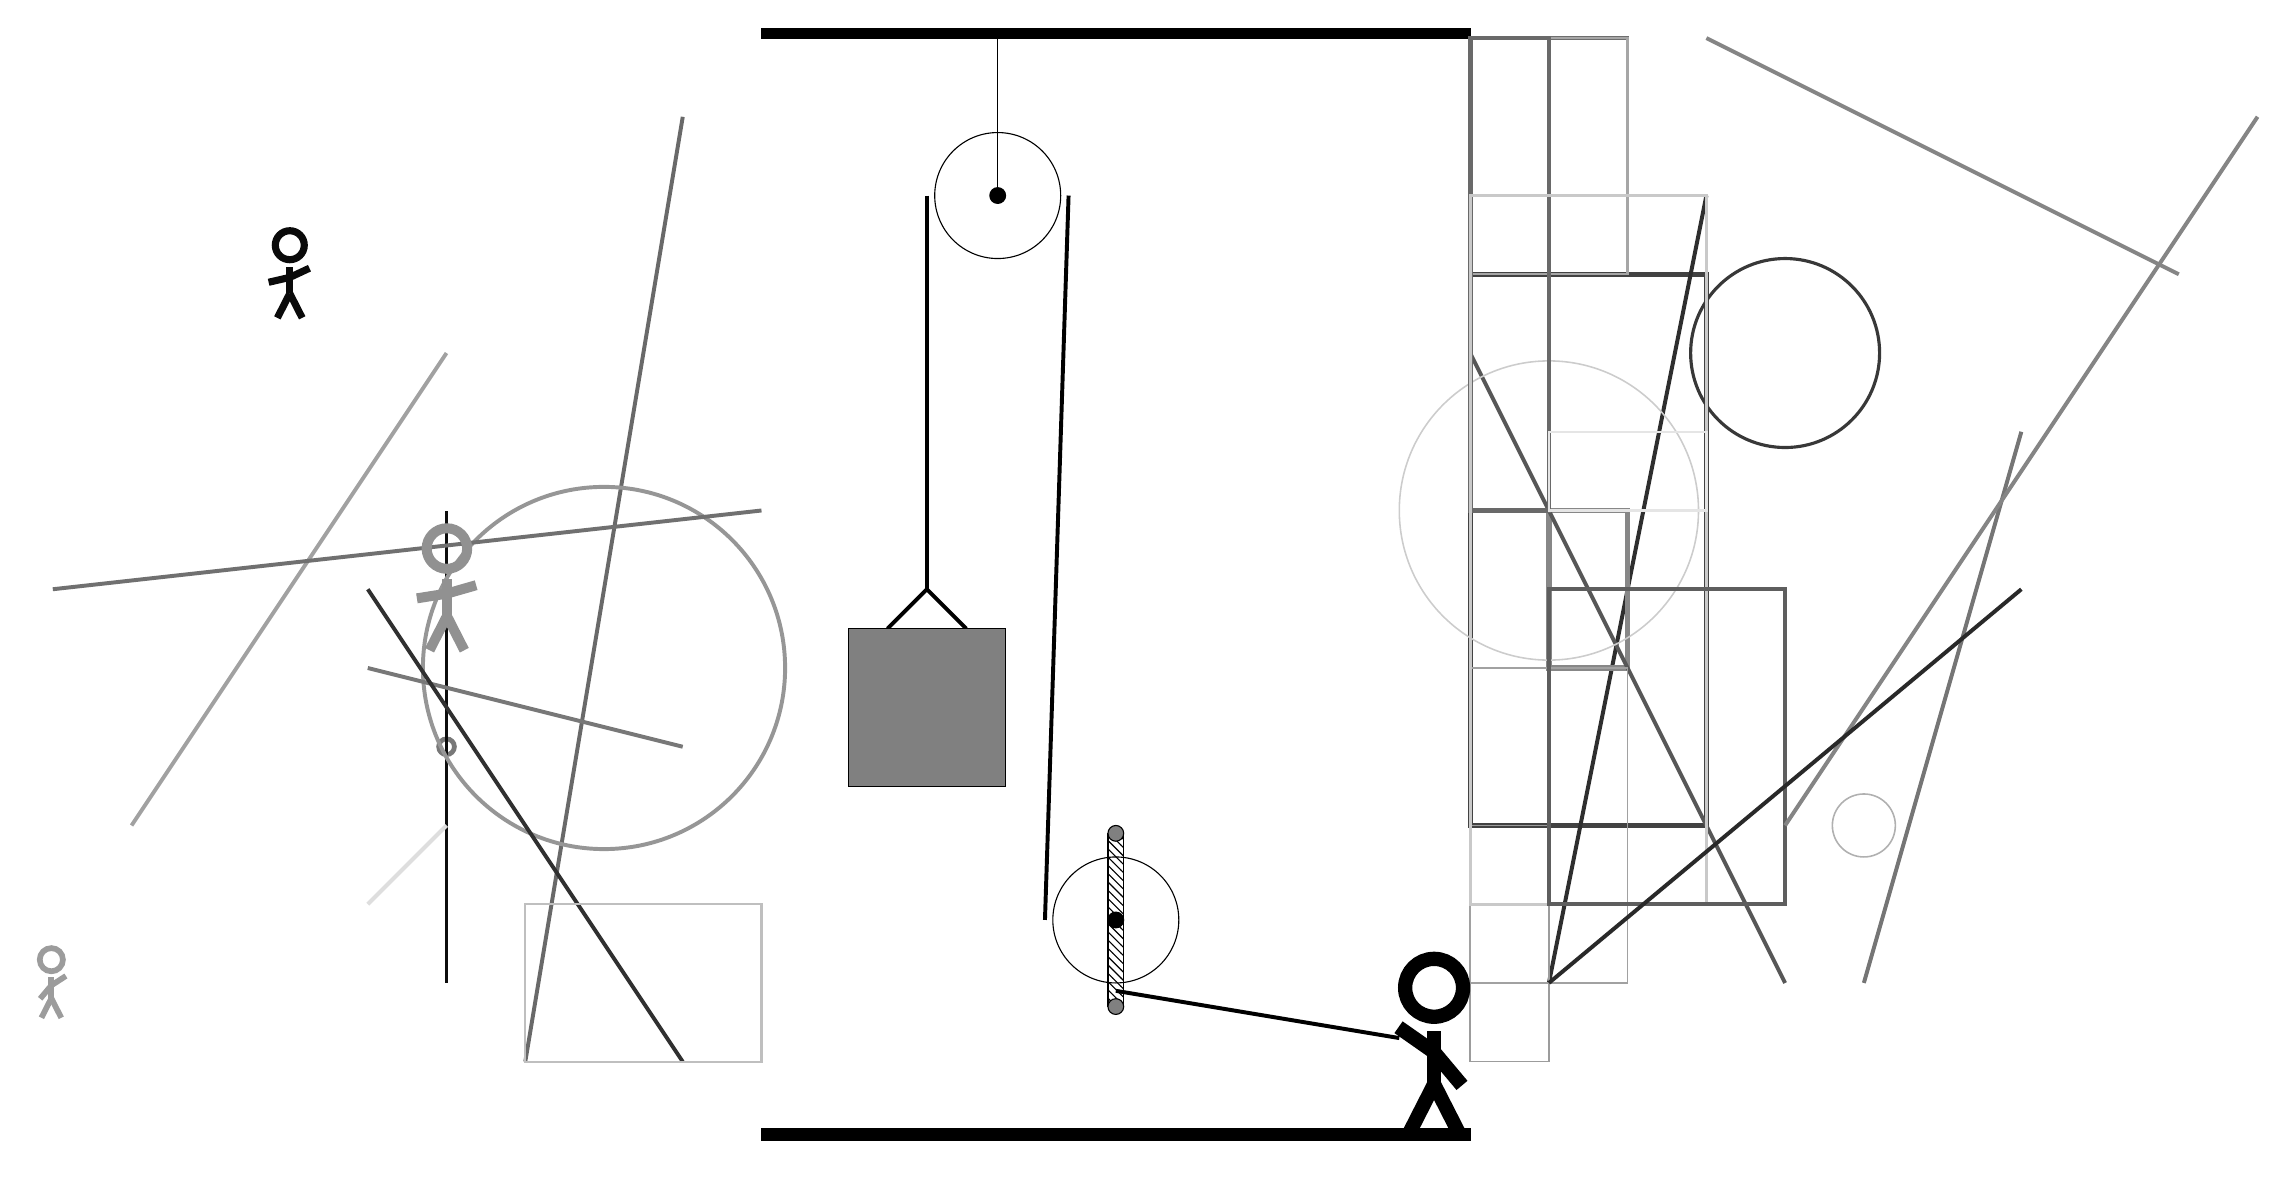
\begin{tikzpicture}
			%%%%% START %%%%%
			
			\draw[fill=black] (-2, 14) rectangle (7, 14.125);
			
			\node[line width=0.6mm, color=black!39] at (-11, 2) {\Strichmaxerl[4][50][33]};
			
			\draw[line width=0.4mm, color=black!57] (8, 14) rectangle (9, 11);
			\draw[line width=0.6mm, color=black!74] (7, 4) rectangle (10, 11);
			\draw [line width=0.4mm, color=black!78](11, 10) circle (1.2);
			
			\draw [line width=0.6mm, color=black!53](-6, 5) circle (0.1);
			\draw[line width=0.5mm, color=black!82](8, 2) -- (10, 12);
			\draw[line width=0.7mm, color=black!47] (8, 8) rectangle (9, 6);
			
			\draw[line width=0.5mm, color=black!66](11, 2) -- (7, 10);
			\draw [line width=0.2mm, color=black!31](12, 4) circle (0.4);
			\draw[line width=0.5mm, color=black!95](-6, 2) -- (-6, 8);
			\draw[line width=0.5mm, color=black!59](-5, 1) -- (-3, 13);
			\draw [line width=0.5mm, color=black!41](-4, 6) circle (2.3);
			\draw [line width=0.2mm, color=black!20](8, 8) circle (1.9);
			
			\draw[line width=0.5mm, color=black!48](10, 14) -- (16, 11);
			\draw[line width=0.2mm, color=black!39] (8, 4) rectangle (7, 1);
			\draw[line width=0.2mm, color=black!37] (9, 6) rectangle (7, 2);
			\draw[line width=0.5mm, color=black!53](-3, 5) -- (-7, 6);
			\draw[line width=0.5mm, color=black!54](12, 2) -- (14, 9);
			\draw[line width=0.5mm, color=black!37](-6, 10) -- (-10, 4);
			\draw[line width=0.3mm, color=black!35] (7, 11) rectangle (9, 14);
			\draw[line width=0.5mm, color=black!81](-3, 1) -- (-7, 7);
			
			\draw[line width=0.6mm, color=black!59] (8, 14) rectangle (7, 8);
			\draw[line width=0.5mm, color=black!56](-2, 8) -- (-11, 7);
			\draw[line width=0.5mm, color=black!13](-6, 4) -- (-7, 3);
			\draw[line width=0.4mm, color=black!21] (7, 12) rectangle (10, 3);
			
			\node[line width=0.7mm, color=black!43] at (-6, 7) {\Strichmaxerl[7][9][16]};
			\draw[line width=0.3mm, color=black!10] (8, 8) rectangle (10, 9);
			\draw[line width=0.5mm, color=black!63] (8, 3) rectangle (11, 7);
			\draw[line width=0.3mm, color=black!25] (-2, 1) rectangle (-5, 3);
			\draw[line width=0.5mm, color=black!48](11, 4) -- (17, 13);
			\draw[line width=0.5mm, color=black!84](8, 2) -- (14, 7);
			
			\node[line width=0.3mm, color=black!96] at (-8, 11) {\Strichmaxerl[5][13][25]};
			
			\draw (1, 12) circle (0.8);
			\draw[fill=black] (1, 12) circle (0.1);
			\draw (1, 14) -- (1, 12);
			
			\draw[fill=white](2.5, 2.8) circle (0.8);
			\draw[fill=black] (2.5, 2.8) circle (0.1);
			\draw[pattern=north west lines, pattern color=black] (2.4, 3.9) rectangle (2.6, 1.7);
			\draw[fill=black!50] (2.5, 3.9) circle (0.1);
			\draw[fill=black!50] (2.5, 1.7) circle (0.1);
			
			\draw[line width=0.5mm] (-0.4, 6.5) -- (0.1, 7.0) -- (0.6, 6.5);
			\draw[fill=black!50] (-0.9, 6.5) rectangle (1.1, 4.5);
			
			\draw[line width=0.5mm] (0.1, 12) -- (0.1, 7.0);
			\centerarc[line width=0.5mm](1, 12)(0:180:0.9);
			\draw[line width=0.5mm](1.9, 12) -- (1.6, 2.8);
			\centerarc[line width=0.5mm](2.5, 2.8)(180:270:0.9);
			\draw[line width=0.5mm](2.5, 1.9) -- (6.1, 1.3);
			
			\node at (6.5, 1.2) {\Strichmaxerl[10][-35][-50]};
			
			\draw[fill=black] (-2, 0) rectangle (7, 0.15);
			
			%%%%% END %%%%%
		\end{tikzpicture}
	\end{figure}	
\end{document}